\documentclass[usenames,dvipsnames]{article} % For LaTeX2e
\usepackage{iclr2022_conference,times}

% Optional math commands from https://github.com/goodfeli/dlbook_notation.
%%%%% NEW MATH DEFINITIONS %%%%%

\usepackage{amsmath,amsfonts,bm}

% Mark sections of captions for referring to divisions of figures
\newcommand{\figleft}{{\em (Left)}}
\newcommand{\figcenter}{{\em (Center)}}
\newcommand{\figright}{{\em (Right)}}
\newcommand{\figtop}{{\em (Top)}}
\newcommand{\figbottom}{{\em (Bottom)}}
\newcommand{\captiona}{{\em (a)}}
\newcommand{\captionb}{{\em (b)}}
\newcommand{\captionc}{{\em (c)}}
\newcommand{\captiond}{{\em (d)}}

% Highlight a newly defined term
\newcommand{\newterm}[1]{{\bf #1}}


% Figure reference, lower-case.
\def\figref#1{figure~\ref{#1}}
% Figure reference, capital. For start of sentence
\def\Figref#1{Figure~\ref{#1}}
\def\twofigref#1#2{figures \ref{#1} and \ref{#2}}
\def\quadfigref#1#2#3#4{figures \ref{#1}, \ref{#2}, \ref{#3} and \ref{#4}}
% Section reference, lower-case.
\def\secref#1{section~\ref{#1}}
% Section reference, capital.
\def\Secref#1{Section~\ref{#1}}
% Reference to two sections.
\def\twosecrefs#1#2{sections \ref{#1} and \ref{#2}}
% Reference to three sections.
\def\secrefs#1#2#3{sections \ref{#1}, \ref{#2} and \ref{#3}}
% Reference to an equation, lower-case.
\def\eqref#1{equation~\ref{#1}}
% Reference to an equation, upper case
\def\Eqref#1{Equation~\ref{#1}}
% A raw reference to an equation---avoid using if possible
\def\plaineqref#1{\ref{#1}}
% Reference to a chapter, lower-case.
\def\chapref#1{chapter~\ref{#1}}
% Reference to an equation, upper case.
\def\Chapref#1{Chapter~\ref{#1}}
% Reference to a range of chapters
\def\rangechapref#1#2{chapters\ref{#1}--\ref{#2}}
% Reference to an algorithm, lower-case.
\def\algref#1{algorithm~\ref{#1}}
% Reference to an algorithm, upper case.
\def\Algref#1{Algorithm~\ref{#1}}
\def\twoalgref#1#2{algorithms \ref{#1} and \ref{#2}}
\def\Twoalgref#1#2{Algorithms \ref{#1} and \ref{#2}}
% Reference to a part, lower case
\def\partref#1{part~\ref{#1}}
% Reference to a part, upper case
\def\Partref#1{Part~\ref{#1}}
\def\twopartref#1#2{parts \ref{#1} and \ref{#2}}

\def\ceil#1{\lceil #1 \rceil}
\def\floor#1{\lfloor #1 \rfloor}
\def\1{\bm{1}}
\newcommand{\train}{\mathcal{D}}
\newcommand{\valid}{\mathcal{D_{\mathrm{valid}}}}
\newcommand{\test}{\mathcal{D_{\mathrm{test}}}}

\def\eps{{\epsilon}}


% Random variables
\def\reta{{\textnormal{$\eta$}}}
\def\ra{{\textnormal{a}}}
\def\rb{{\textnormal{b}}}
\def\rc{{\textnormal{c}}}
\def\rd{{\textnormal{d}}}
\def\re{{\textnormal{e}}}
\def\rf{{\textnormal{f}}}
\def\rg{{\textnormal{g}}}
\def\rh{{\textnormal{h}}}
\def\ri{{\textnormal{i}}}
\def\rj{{\textnormal{j}}}
\def\rk{{\textnormal{k}}}
\def\rl{{\textnormal{l}}}
% rm is already a command, just don't name any random variables m
\def\rn{{\textnormal{n}}}
\def\ro{{\textnormal{o}}}
\def\rp{{\textnormal{p}}}
\def\rq{{\textnormal{q}}}
\def\rr{{\textnormal{r}}}
\def\rs{{\textnormal{s}}}
\def\rt{{\textnormal{t}}}
\def\ru{{\textnormal{u}}}
\def\rv{{\textnormal{v}}}
\def\rw{{\textnormal{w}}}
\def\rx{{\textnormal{x}}}
\def\ry{{\textnormal{y}}}
\def\rz{{\textnormal{z}}}

% Random vectors
\def\rvepsilon{{\mathbf{\epsilon}}}
\def\rvtheta{{\mathbf{\theta}}}
\def\rva{{\mathbf{a}}}
\def\rvb{{\mathbf{b}}}
\def\rvc{{\mathbf{c}}}
\def\rvd{{\mathbf{d}}}
\def\rve{{\mathbf{e}}}
\def\rvf{{\mathbf{f}}}
\def\rvg{{\mathbf{g}}}
\def\rvh{{\mathbf{h}}}
\def\rvu{{\mathbf{i}}}
\def\rvj{{\mathbf{j}}}
\def\rvk{{\mathbf{k}}}
\def\rvl{{\mathbf{l}}}
\def\rvm{{\mathbf{m}}}
\def\rvn{{\mathbf{n}}}
\def\rvo{{\mathbf{o}}}
\def\rvp{{\mathbf{p}}}
\def\rvq{{\mathbf{q}}}
\def\rvr{{\mathbf{r}}}
\def\rvs{{\mathbf{s}}}
\def\rvt{{\mathbf{t}}}
\def\rvu{{\mathbf{u}}}
\def\rvv{{\mathbf{v}}}
\def\rvw{{\mathbf{w}}}
\def\rvx{{\mathbf{x}}}
\def\rvy{{\mathbf{y}}}
\def\rvz{{\mathbf{z}}}

% Elements of random vectors
\def\erva{{\textnormal{a}}}
\def\ervb{{\textnormal{b}}}
\def\ervc{{\textnormal{c}}}
\def\ervd{{\textnormal{d}}}
\def\erve{{\textnormal{e}}}
\def\ervf{{\textnormal{f}}}
\def\ervg{{\textnormal{g}}}
\def\ervh{{\textnormal{h}}}
\def\ervi{{\textnormal{i}}}
\def\ervj{{\textnormal{j}}}
\def\ervk{{\textnormal{k}}}
\def\ervl{{\textnormal{l}}}
\def\ervm{{\textnormal{m}}}
\def\ervn{{\textnormal{n}}}
\def\ervo{{\textnormal{o}}}
\def\ervp{{\textnormal{p}}}
\def\ervq{{\textnormal{q}}}
\def\ervr{{\textnormal{r}}}
\def\ervs{{\textnormal{s}}}
\def\ervt{{\textnormal{t}}}
\def\ervu{{\textnormal{u}}}
\def\ervv{{\textnormal{v}}}
\def\ervw{{\textnormal{w}}}
\def\ervx{{\textnormal{x}}}
\def\ervy{{\textnormal{y}}}
\def\ervz{{\textnormal{z}}}

% Random matrices
\def\rmA{{\mathbf{A}}}
\def\rmB{{\mathbf{B}}}
\def\rmC{{\mathbf{C}}}
\def\rmD{{\mathbf{D}}}
\def\rmE{{\mathbf{E}}}
\def\rmF{{\mathbf{F}}}
\def\rmG{{\mathbf{G}}}
\def\rmH{{\mathbf{H}}}
\def\rmI{{\mathbf{I}}}
\def\rmJ{{\mathbf{J}}}
\def\rmK{{\mathbf{K}}}
\def\rmL{{\mathbf{L}}}
\def\rmM{{\mathbf{M}}}
\def\rmN{{\mathbf{N}}}
\def\rmO{{\mathbf{O}}}
\def\rmP{{\mathbf{P}}}
\def\rmQ{{\mathbf{Q}}}
\def\rmR{{\mathbf{R}}}
\def\rmS{{\mathbf{S}}}
\def\rmT{{\mathbf{T}}}
\def\rmU{{\mathbf{U}}}
\def\rmV{{\mathbf{V}}}
\def\rmW{{\mathbf{W}}}
\def\rmX{{\mathbf{X}}}
\def\rmY{{\mathbf{Y}}}
\def\rmZ{{\mathbf{Z}}}

% Elements of random matrices
\def\ermA{{\textnormal{A}}}
\def\ermB{{\textnormal{B}}}
\def\ermC{{\textnormal{C}}}
\def\ermD{{\textnormal{D}}}
\def\ermE{{\textnormal{E}}}
\def\ermF{{\textnormal{F}}}
\def\ermG{{\textnormal{G}}}
\def\ermH{{\textnormal{H}}}
\def\ermI{{\textnormal{I}}}
\def\ermJ{{\textnormal{J}}}
\def\ermK{{\textnormal{K}}}
\def\ermL{{\textnormal{L}}}
\def\ermM{{\textnormal{M}}}
\def\ermN{{\textnormal{N}}}
\def\ermO{{\textnormal{O}}}
\def\ermP{{\textnormal{P}}}
\def\ermQ{{\textnormal{Q}}}
\def\ermR{{\textnormal{R}}}
\def\ermS{{\textnormal{S}}}
\def\ermT{{\textnormal{T}}}
\def\ermU{{\textnormal{U}}}
\def\ermV{{\textnormal{V}}}
\def\ermW{{\textnormal{W}}}
\def\ermX{{\textnormal{X}}}
\def\ermY{{\textnormal{Y}}}
\def\ermZ{{\textnormal{Z}}}

% Vectors
\def\vzero{{\bm{0}}}
\def\vone{{\bm{1}}}
\def\vmu{{\bm{\mu}}}
\def\vtheta{{\bm{\theta}}}
\def\va{{\bm{a}}}
\def\vb{{\bm{b}}}
\def\vc{{\bm{c}}}
\def\vd{{\bm{d}}}
\def\ve{{\bm{e}}}
\def\vf{{\bm{f}}}
\def\vg{{\bm{g}}}
\def\vh{{\bm{h}}}
\def\vi{{\bm{i}}}
\def\vj{{\bm{j}}}
\def\vk{{\bm{k}}}
\def\vl{{\bm{l}}}
\def\vm{{\bm{m}}}
\def\vn{{\bm{n}}}
\def\vo{{\bm{o}}}
\def\vp{{\bm{p}}}
\def\vq{{\bm{q}}}
\def\vr{{\bm{r}}}
\def\vs{{\bm{s}}}
\def\vt{{\bm{t}}}
\def\vu{{\bm{u}}}
\def\vv{{\bm{v}}}
\def\vw{{\bm{w}}}
\def\vx{{\bm{x}}}
\def\vy{{\bm{y}}}
\def\vz{{\bm{z}}}

% Elements of vectors
\def\evalpha{{\alpha}}
\def\evbeta{{\beta}}
\def\evepsilon{{\epsilon}}
\def\evlambda{{\lambda}}
\def\evomega{{\omega}}
\def\evmu{{\mu}}
\def\evpsi{{\psi}}
\def\evsigma{{\sigma}}
\def\evtheta{{\theta}}
\def\eva{{a}}
\def\evb{{b}}
\def\evc{{c}}
\def\evd{{d}}
\def\eve{{e}}
\def\evf{{f}}
\def\evg{{g}}
\def\evh{{h}}
\def\evi{{i}}
\def\evj{{j}}
\def\evk{{k}}
\def\evl{{l}}
\def\evm{{m}}
\def\evn{{n}}
\def\evo{{o}}
\def\evp{{p}}
\def\evq{{q}}
\def\evr{{r}}
\def\evs{{s}}
\def\evt{{t}}
\def\evu{{u}}
\def\evv{{v}}
\def\evw{{w}}
\def\evx{{x}}
\def\evy{{y}}
\def\evz{{z}}

% Matrix
\def\mA{{\bm{A}}}
\def\mB{{\bm{B}}}
\def\mC{{\bm{C}}}
\def\mD{{\bm{D}}}
\def\mE{{\bm{E}}}
\def\mF{{\bm{F}}}
\def\mG{{\bm{G}}}
\def\mH{{\bm{H}}}
\def\mI{{\bm{I}}}
\def\mJ{{\bm{J}}}
\def\mK{{\bm{K}}}
\def\mL{{\bm{L}}}
\def\mM{{\bm{M}}}
\def\mN{{\bm{N}}}
\def\mO{{\bm{O}}}
\def\mP{{\bm{P}}}
\def\mQ{{\bm{Q}}}
\def\mR{{\bm{R}}}
\def\mS{{\bm{S}}}
\def\mT{{\bm{T}}}
\def\mU{{\bm{U}}}
\def\mV{{\bm{V}}}
\def\mW{{\bm{W}}}
\def\mX{{\bm{X}}}
\def\mY{{\bm{Y}}}
\def\mZ{{\bm{Z}}}
\def\mBeta{{\bm{\beta}}}
\def\mPhi{{\bm{\Phi}}}
\def\mLambda{{\bm{\Lambda}}}
\def\mSigma{{\bm{\Sigma}}}

% Tensor
\DeclareMathAlphabet{\mathsfit}{\encodingdefault}{\sfdefault}{m}{sl}
\SetMathAlphabet{\mathsfit}{bold}{\encodingdefault}{\sfdefault}{bx}{n}
\newcommand{\tens}[1]{\bm{\mathsfit{#1}}}
\def\tA{{\tens{A}}}
\def\tB{{\tens{B}}}
\def\tC{{\tens{C}}}
\def\tD{{\tens{D}}}
\def\tE{{\tens{E}}}
\def\tF{{\tens{F}}}
\def\tG{{\tens{G}}}
\def\tH{{\tens{H}}}
\def\tI{{\tens{I}}}
\def\tJ{{\tens{J}}}
\def\tK{{\tens{K}}}
\def\tL{{\tens{L}}}
\def\tM{{\tens{M}}}
\def\tN{{\tens{N}}}
\def\tO{{\tens{O}}}
\def\tP{{\tens{P}}}
\def\tQ{{\tens{Q}}}
\def\tR{{\tens{R}}}
\def\tS{{\tens{S}}}
\def\tT{{\tens{T}}}
\def\tU{{\tens{U}}}
\def\tV{{\tens{V}}}
\def\tW{{\tens{W}}}
\def\tX{{\tens{X}}}
\def\tY{{\tens{Y}}}
\def\tZ{{\tens{Z}}}


% Graph
\def\gA{{\mathcal{A}}}
\def\gB{{\mathcal{B}}}
\def\gC{{\mathcal{C}}}
\def\gD{{\mathcal{D}}}
\def\gE{{\mathcal{E}}}
\def\gF{{\mathcal{F}}}
\def\gG{{\mathcal{G}}}
\def\gH{{\mathcal{H}}}
\def\gI{{\mathcal{I}}}
\def\gJ{{\mathcal{J}}}
\def\gK{{\mathcal{K}}}
\def\gL{{\mathcal{L}}}
\def\gM{{\mathcal{M}}}
\def\gN{{\mathcal{N}}}
\def\gO{{\mathcal{O}}}
\def\gP{{\mathcal{P}}}
\def\gQ{{\mathcal{Q}}}
\def\gR{{\mathcal{R}}}
\def\gS{{\mathcal{S}}}
\def\gT{{\mathcal{T}}}
\def\gU{{\mathcal{U}}}
\def\gV{{\mathcal{V}}}
\def\gW{{\mathcal{W}}}
\def\gX{{\mathcal{X}}}
\def\gY{{\mathcal{Y}}}
\def\gZ{{\mathcal{Z}}}

% Sets
\def\sA{{\mathbb{A}}}
\def\sB{{\mathbb{B}}}
\def\sC{{\mathbb{C}}}
\def\sD{{\mathbb{D}}}
% Don't use a set called E, because this would be the same as our symbol
% for expectation.
\def\sF{{\mathbb{F}}}
\def\sG{{\mathbb{G}}}
\def\sH{{\mathbb{H}}}
\def\sI{{\mathbb{I}}}
\def\sJ{{\mathbb{J}}}
\def\sK{{\mathbb{K}}}
\def\sL{{\mathbb{L}}}
\def\sM{{\mathbb{M}}}
\def\sN{{\mathbb{N}}}
\def\sO{{\mathbb{O}}}
\def\sP{{\mathbb{P}}}
\def\sQ{{\mathbb{Q}}}
\def\sR{{\mathbb{R}}}
\def\sS{{\mathbb{S}}}
\def\sT{{\mathbb{T}}}
\def\sU{{\mathbb{U}}}
\def\sV{{\mathbb{V}}}
\def\sW{{\mathbb{W}}}
\def\sX{{\mathbb{X}}}
\def\sY{{\mathbb{Y}}}
\def\sZ{{\mathbb{Z}}}

% Entries of a matrix
\def\emLambda{{\Lambda}}
\def\emA{{A}}
\def\emB{{B}}
\def\emC{{C}}
\def\emD{{D}}
\def\emE{{E}}
\def\emF{{F}}
\def\emG{{G}}
\def\emH{{H}}
\def\emI{{I}}
\def\emJ{{J}}
\def\emK{{K}}
\def\emL{{L}}
\def\emM{{M}}
\def\emN{{N}}
\def\emO{{O}}
\def\emP{{P}}
\def\emQ{{Q}}
\def\emR{{R}}
\def\emS{{S}}
\def\emT{{T}}
\def\emU{{U}}
\def\emV{{V}}
\def\emW{{W}}
\def\emX{{X}}
\def\emY{{Y}}
\def\emZ{{Z}}
\def\emSigma{{\Sigma}}

% entries of a tensor
% Same font as tensor, without \bm wrapper
\newcommand{\etens}[1]{\mathsfit{#1}}
\def\etLambda{{\etens{\Lambda}}}
\def\etA{{\etens{A}}}
\def\etB{{\etens{B}}}
\def\etC{{\etens{C}}}
\def\etD{{\etens{D}}}
\def\etE{{\etens{E}}}
\def\etF{{\etens{F}}}
\def\etG{{\etens{G}}}
\def\etH{{\etens{H}}}
\def\etI{{\etens{I}}}
\def\etJ{{\etens{J}}}
\def\etK{{\etens{K}}}
\def\etL{{\etens{L}}}
\def\etM{{\etens{M}}}
\def\etN{{\etens{N}}}
\def\etO{{\etens{O}}}
\def\etP{{\etens{P}}}
\def\etQ{{\etens{Q}}}
\def\etR{{\etens{R}}}
\def\etS{{\etens{S}}}
\def\etT{{\etens{T}}}
\def\etU{{\etens{U}}}
\def\etV{{\etens{V}}}
\def\etW{{\etens{W}}}
\def\etX{{\etens{X}}}
\def\etY{{\etens{Y}}}
\def\etZ{{\etens{Z}}}

% The true underlying data generating distribution
\newcommand{\pdata}{p_{\rm{data}}}
% The empirical distribution defined by the training set
\newcommand{\ptrain}{\hat{p}_{\rm{data}}}
\newcommand{\Ptrain}{\hat{P}_{\rm{data}}}
% The model distribution
\newcommand{\pmodel}{p_{\rm{model}}}
\newcommand{\Pmodel}{P_{\rm{model}}}
\newcommand{\ptildemodel}{\tilde{p}_{\rm{model}}}
% Stochastic autoencoder distributions
\newcommand{\pencode}{p_{\rm{encoder}}}
\newcommand{\pdecode}{p_{\rm{decoder}}}
\newcommand{\precons}{p_{\rm{reconstruct}}}

\newcommand{\laplace}{\mathrm{Laplace}} % Laplace distribution

\newcommand{\E}{\mathbb{E}}
\newcommand{\Ls}{\mathcal{L}}
\newcommand{\R}{\mathbb{R}}
\newcommand{\emp}{\tilde{p}}
\newcommand{\lr}{\alpha}
\newcommand{\reg}{\lambda}
\newcommand{\rect}{\mathrm{rectifier}}
\newcommand{\softmax}{\mathrm{softmax}}
\newcommand{\sigmoid}{\sigma}
\newcommand{\softplus}{\zeta}
\newcommand{\KL}{D_{\mathrm{KL}}}
\newcommand{\Var}{\mathrm{Var}}
\newcommand{\standarderror}{\mathrm{SE}}
\newcommand{\Cov}{\mathrm{Cov}}
% Wolfram Mathworld says $L^2$ is for function spaces and $\ell^2$ is for vectors
% But then they seem to use $L^2$ for vectors throughout the site, and so does
% wikipedia.
\newcommand{\normlzero}{L^0}
\newcommand{\normlone}{L^1}
\newcommand{\normltwo}{L^2}
\newcommand{\normlp}{L^p}
\newcommand{\normmax}{L^\infty}

\newcommand{\parents}{Pa} % See usage in notation.tex. Chosen to match Daphne's book.

\DeclareMathOperator*{\argmax}{arg\,max}
\DeclareMathOperator*{\argmin}{arg\,min}

\DeclareMathOperator{\sign}{sign}
\DeclareMathOperator{\Tr}{Tr}
\let\ab\allowbreak


% Packages
\usepackage{multirow}
\usepackage{graphicx}
\usepackage{hyperref}
\usepackage{float}

\usepackage{pgfplots, pgfplotstable}
\usepgfplotslibrary{fillbetween}
\usepackage[pdf]{graphviz}
\usepackage{tikz}
\usepackage{enumitem}
\usepgfplotslibrary{statistics}

\usepackage{booktabs}
\usepackage{pifont}
\usepackage{fontawesome}

\newcommand{\wmark}{\textcolor{orange}{\ding{45}}}
\newcommand{\cmark}{\textcolor{green!80!black}{\ding{51}}}
\newcommand{\xmark}{\textcolor{red}{\ding{55}}}

\usepackage{multicol}

\usepackage{bussproofs}
\usepackage{stackengine}
\usepackage{amssymb}

% Packages
\usepackage{soul}
\usepackage{listings}
\usepackage{xcolor}
\DeclareRobustCommand{\hlred}[1]{{\sethlcolor{pink}\hl{#1}}}
\usepackage{fontspec}

\setmonofont{JetBrainsMono}[
  Contextuals={Alternate},
  Path=./JetBrainsFontFiles/,
  Extension = .ttf,
  UprightFont=*-Regular,
  BoldFont=*-Bold,
  ItalicFont=*-Italic,
  BoldItalicFont=*-BoldItalic
]

\makeatletter
\def\verbatim@nolig@list{}
\makeatother

\lstdefinelanguage{kotlin}{
  comment=[l]{//},
  commentstyle={\color{gray}\ttfamily},
  emph={delegate, filter, firstOrNull, forEach, it, lazy, mapNotNull, println, repeat, assert, with, head, tail, len, return@},
  numberstyle=\noncopyable,
  emphstyle={\color{OrangeRed}},
  identifierstyle=\color{black},
  keywords={abstract, actual, as, as?, break, by, class, companion, continue, data, do, dynamic, else, enum, expect, false, final, for, fun, get, if, import, in, infix, interface, internal, is, null, object, open, operator, override, package, private, public, return, sealed, set, super, suspend, this, throw, true, try, catch, typealias, val, var, vararg, when, where, while, tailrec, reified},
  keywordstyle={\color{NavyBlue}\bfseries},
  morecomment=[s]{/*}{*/},
  morestring=[b]",
  morestring=[s]{"""*}{*"""},
  ndkeywords={@Deprecated, @JvmField, @JvmName, @JvmOverloads, @JvmStatic, @JvmSynthetic, Array, Byte, Double, Float, Boolean, Int, Integer, Iterable, Long, Runnable, Short, String, int},
  ndkeywordstyle={\color{BurntOrange}\bfseries},
  sensitive=true,
  stringstyle={\color{ForestGreen}\ttfamily},
  literate={`}{{\char0}}1,
  escapeinside={(*@}{@*)}
}

\lstset{basicstyle=\ttfamily\lst@ifdisplaystyle\tiny\fi, language=kotlin}


\usepackage{url}
\usepackage{textcomp}


\title{How Robust Are Neural Code Completion Models to Term Rewriting?}
\author{Breandan Considine, Xiaojie Xu, Xujie Si, Jin L.C. Guo\\
\texttt{\{breandan.considine, xiaojie.xu, xsi, jguo\}@\{mail, cs\}.mcgill.ca}\\
}

% The \author macro works with any number of authors. There are two commands
% used to separate the names and addresses of multiple authors: \And and \AND.
%
% Using \And between authors leaves it to \LaTeX{} to determine where to break
% the lines. Using \AND forces a linebreak at that point. So, if \LaTeX{}
% puts 3 of 4 authors names on the first line, and the last on the second
% line, try using \AND instead of \And before the third author name.

\newcommand{\fix}{\marginpar{FIX}}
\newcommand{\new}{\marginpar{NEW}}

%\iclrfinalcopy % Uncomment for camera-ready version, but NOT for submission.
\begin{document}


  \maketitle

  \begin{abstract}
    Neural language models hold great promise as tools for computer-aided programming, but come with certain risks. In the domain of natural language, prior work has revealed these models can be sensitive to naturally-occurring variance and malfunction in unpredictable ways. A more methodical examination of neural language models is necessary to understand their behavior on programming-related tasks. In this work, we develop a methodology for systematically evaluating neural code completion models using common source code rewrites. Applying these synthetic rewrites to a dataset of handwritten source code fragments, we obtain results for four pretrained models, which exhibit varying degrees of robustness under transformation. We give preliminary results from those experiments and discuss our approach to testing pretrained neural code completion models. Our analysis provides insights into the strengths and weaknesses of different models, and can serve as a foundation for future work for improving the accuracy and robustness of neural code completion models.
  \end{abstract}

  \section{Introduction}\label{sec:introduction}

  Neural language models play an increasingly synergistic role in software engineering, and are featured prominently in recent work on neural code completion~\cite{chen2021evaluating}. Code completion is the task of automatically providing a list of potential completions for some hole in source code. By training a general purpose language model on a large corpus of source code, one can automatically learn programming language syntax, stylistic elements like common variable names as well as more complex features like idioms and natural language documentation. These same models can be adapted to a variety of source-code analysis tasks, such as document synthesis and variable misuse, by strategically placing the holes and conditioning the model's predictions on an appropriate sample space.

  However, there are known risks associated with using neural language models. In the domain of natural language, these models can be sensitive to naturally-occurring variance and malfunction in unpredictable ways when applied to tasks such as interactive dialog and machine translation. In the case of code completion, a model may perform well on a training corpus that is syntactically well-formed and free of errors, but struggle when applied to a corpus containing errors or unfamiliar design patterns. This phenomena is broadly known as `domain mismatch' or `overfitting', and can be quantified by various robustness metrics.

  The robustness of neural language models has been well-studied through the lens of natural language processing (NLP). However, there has been relatively little work on understanding how these models perform on programming-related tasks. In this paper, we aim to fill this gap by developing a methodology for systematically evaluating neural code completion models using semantically-preserving source code transformations. We define a set of code transformations that are commonly used in programming, and measure the distributional shift introduced by applying them to a dataset of handwritten source code fragments. We evaluate the same set of transformations across four pretrained language models and three downstream tasks. Our results provide insights into the strengths and weaknesses of those models, and serve as a foundation for future work towards improving the accuracy and robustness of neural code completion via dataset engineering.

  \section{Background}\label{sec:background}

  The same program can be written in many possible ways. Often, those variants contain superficial changes to the source code, but do not meaningfully alter the behavior of the underlying program. In the same way that skilled programmers should be flexible to rewriting, one would expect a code completion model in a language semantically invariant to certain rewrites to exhibit invariance under those same rewrites. As we will demonstrate, this property may not necessarily hold in general.

  For example, let $\textsc{Code} := \lstinline|int old = 0; while (<mask> < 10) {...}|$ and assume we have a pretrained language model $\mathcal{M}_\theta: \lstinline|String|\rightarrow\lstinline|String|$ which gives the completion:

  \begin{equation}
    \mathcal{M}_\theta[\textsc{Code}] \vdash \textsc{Code}\:\{\texttt{<mask>} \rightarrow \:\texttt{old}\}
  \end{equation}

  If we then rename the variable \texttt{old} to \texttt{fresh} inside the fragment \textsc{Code}, we would expect our language model's completion to shift in kind, a property we call \textit{name equivariance}:

  \begin{center}
    \begin{prooftree}
      \AxiomC{Γ \vdash \:$\mathcal{M}_{\theta}$}
      \AxiomC{\textsc{Code}}
      \AxiomC{\{\texttt{old} \rightarrow\:\texttt{fresh}\}: \lstinline|String| → \lstinline|String|}
      \RightLabel{\textsc{NameEquivariance}}
      \TrinaryInfC{$\Gamma \vdash \mathcal{M}_{\theta}[\textsc{Code}\:\{\texttt{old} \rightarrow\:\texttt{fresh}\}] = \mathcal{M}_{\theta}[\textsc{Code}]\{\texttt{old} \rightarrow\:\texttt{fresh}\}$}
    \end{prooftree}
  \end{center}

As documented by prior literature, neural language models can be prone to semantic drift that is not supported by the underlying language semantics. The question becomes, how do we estimate the robustness of those models to rewrites which are known \textit{a priori} to be cosmetic in nature? In our work, we address this question by identifying four classes of cosmetic rewrites, apply them to a dataset of Java source code, and measure the relative drift of four SoTA pretrained language models across three separate code completion tasks.

The paper is structured as follows. In Sec.~\ref{sec:background}, we give some background on the methods and problem at hand. In Sec.~\ref{sec:related_work} we give some related work. In Sec.~\ref{sec:method}, we describe our method. In Sec.~\ref{sec:results} we give some results and discuss their implications. Finally, in Sec. ~\ref{sec:conclusion} we give some concluding remarks. Our results are fully reproducible and can be found at: \url{https://anonymous.4open.science/r/cstk-1458}.



First conceived in the software testing literature, metamorphic testing~\cite{chen1995metamorphic} is a concept known in machine learning as \textit{self-supervision}. In settings where labels are scarce but invariant to certain groups of transformation or \textit{metamorphic relations}, given a finite labeled dataset, one can generate an effectively limitless quantity of synthetic data by selecting and recombining those transformations in an orderly manner. For example, computer vision models should be invariant to shift, scale and rotation: given a small dataset of labeled images, we can apply these transformations to generate much larger training or validation set. Could similar kinds of transformations exist for code?

  \section{Related Work}\label{sec:related_work}

 Recent work in neural language modeling has shown impressive progress in long-range sequence prediction, starting with self-attention~\citep{vaswani2017attention}, to the BERT~\citep{devlin2018bert} and RoBERTa~\citep{liu2019roberta} architectures, now widely available in neural code completion models such as CodeBERT~\citep{feng2020codebert} and GraphCodeBERT~\citep{guo2021graphcodebert}. However these models have known limitations, such as their inability to represent long-term dependencies and their sensitivity to noise in the input space~\cite{sun2020adv}. Similar studies have been undertaken to study the robustness of pretrained language models of source code~\citep{bielik2020adversarial, zhou2021adversarial}. Due to the clear distinction between syntax and semantics in programming languages, one can more precisely reason about semantically admissible perturbations, a task which is considerably more difficult in natural languages. Similar research has been undertaken~\citep{weiss2018practical, chirkova2020empirical, chen2021evaluating} to characterize the families of computational languages neural language models can recognize in practice. Our work builds on this literature from an engineering standpoint: we investigate how neural code completion models respond to plausible cosmetic variation. Applying synthetic transformations to a datatset of naturally-occurring code snippets, we compare the robustness of four SoTA neural language models on three downstream tasks: code completion, document completion, and variable misuse. %We have identified three high-level categories of source code transformations:

%  \begin{enumerate}[itemsep=1ex]
%    \item \textbf{Syntactic}, which may be valid (i.e., parsable) or invalid (e.g., typos, imbalanced parentheses, unparsable code)
%    \item \textbf{Semantic}, either preserving (functional code clones) or altering (e.g., dis-equal constant or expression rewriting)
%    \item \textbf{Cosmetic}, e.g., variable renaming, independent statement reordering, extra documentation, dead code, or logging
%  \end{enumerate}

%  In contrast with syntactic or semantic transformations, cosmetic transformations are semantically identical, syntactically valid and only superficially alter syntactic structure. We show that even in this highly restrictive space of transformations, source code has many degrees of freedom: two authors implementing the same function may select different variable names or other cosmetic features, such as whitespaces, diagnostic statements or comments.  Yet our results suggest that even in this narrow space of transformations, SoTA neural code completion models can be surprisingly sensitive to noise in the cosmetic domain space.


  \section{Method}\label{sec:method}

  We define the following four transformations and examine their effect on language models.

  \begin{center}
      \begin{prooftree}
        \AxiomC{Γ \vdash \:\texttt{function(args)}}
        \AxiomC{$\texttt{function} \not\in \textsc{StandardLibrary}$}
        \RightLabel{\textsc{PermuteArguments}}
        \BinaryInfC{Γ \vdash \:\textsc{Code}\:\{\texttt{function(args)} \rightarrow\:\texttt{function(}\faRandom\texttt{args)}\}}
      \end{prooftree}

      \begin{prooftree}
        \AxiomC{Γ \vdash \,\,\stackanchor{\textvisiblespace\texttt{line\_1;}}{\textvisiblespace\texttt{line\_2;}}}
        \AxiomC{\textsc{Tokens}(\texttt{line\_1}) \cap\:\textsc{Tokens}(\texttt{line\_2}) = \varnothing}
        \RightLabel{\textsc{SwapIndepLines}}
        \BinaryInfC{Γ \vdash \,\,\stackanchor{\textvisiblespace\texttt{line\_2;}}{\textvisiblespace\texttt{line\_1;}}}
      \end{prooftree}

      \begin{prooftree}
        \AxiomC{Γ \vdash \:\texttt{var} \in\:\textsc{ScopedNames}}
        \AxiomC{\stackanchor{\textvisiblespace\texttt{line\_1;}}{\textvisiblespace\texttt{line\_2;}}}
%        \AxiomC{\texttt{print} \not\in\:\textsc{Tokens}(\texttt{line\_1} \:\oplus\, \texttt{line\_2})}
        \RightLabel{\textsc{AddExtraLogging}}
        \BinaryInfC{\Shortstack[l]{{\vphantom{\texttt{line\_1;}}} {Γ \vdash} {\vphantom{\texttt{line\_1;}}}}  \:\Shortstack[l]{{\textvisiblespace\texttt{line\_1;}} {\textvisiblespace\texttt{println("var: \$var");}} {\textvisiblespace\texttt{line\_3;}}}}
      \end{prooftree}

      \begin{prooftree}
        \AxiomC{Γ \vdash \:\texttt{var} \in\:\textsc{ScopedNames}}
        \AxiomC{\texttt{fresh} \in\:\textsc{Synonyms}(\texttt{var}) \setminus\:\textsc{ScopedNames}}
        \RightLabel{\textsc{Rename}}
        \BinaryInfC{Γ \vdash \,\,\textsc{Code}\:\{\:\texttt{var} \rightarrow\:\texttt{fresh}\:\}}
    \end{prooftree}
  \end{center}

  Each task is performed using a special hole-filling strategy and models are scored using a task-appropriate metric.
  We can simulate various kinds of tasks by conditioning on the masked tokens in various ways.
  For single-token completion, we use:

\begin{equation*}
  \text{Precision@1} = \frac{1}{{|\textsc{Tokens}|}}\sum_{\texttt{tok}\in \textsc{Tokens}}\textsc{Model}(\textsc{Code}\:\{\:\texttt{tok}\:\rightarrow\:\texttt{<mask>}\:\}) = \:\textsc{Code}
\end{equation*}

  For document synthesis, we use the following score:

\begin{equation*}
\text{ROUGE-Synonym} = \Delta_{\text{Syn}}(\textsc{Model}^{k}(\textsc{Code}\:\{\:\texttt{//[...]}\:\rightarrow\:\texttt{<mask>}\:\}), \:\texttt{//[...]})
\end{equation*}

  where $\textsc{Model}^{k}$ denotes autoregressively sampling $k$ consecutive tokens, and $\Delta_\text{Syn}$ denotes the synonym overlap between the original and synthetic comments.

  For question answering, e.g., variable misuse, we use mean reciprocal rank (MRR):

\begin{equation*}
\text{MRR} = \frac{1}{|\textsc{Tokens}|} \sum_{\texttt{tok}\in\textsc{Tokens}} \textsc{Rank}\big(\texttt{tok}, \textsc{Model}(\textsc{Code}\:\{\:\texttt{tok}\:\rightarrow\:\texttt{<mask>}\:\}, \textsc{hints})\big)^{-1}
\end{equation*}

  Our dataset consists of a hundred of the highest-starred Java repositories hosted by GitHub organizations with over 100 forks and between 1 and 10 MB in size. This ensures a diverse dataset of active repositories with reasonable quality and stylistic diversity.

  Our goal is to measure the robustness of SoTA neural code completion models on natural code snippets exposed to various cosmetic transformations. To do so, we first construct one SCT from each of the following five categories of cosmetic changes:

  \begin{enumerate}[itemsep=1ex]
    \item \textbf{Synonym renaming}: renames variables with synonyms
    \item \textbf{Peripheral code}: introduces dead code to source code
    \item \textbf{Statement reordering}: swaps independent statements
    \item \textbf{Permute argument order}: scrambles method arguments
  \end{enumerate}

  Ideally, these SCTs would be implemented using a higher-order abstract syntax (HOAS) to ensure syntactic validity, however for the sake of simplicity, we implemented the transformations using a set of ad-hoc regular expressions (regexes). While somewhat clumsy for more complex SCTs, we observed that regex-based pattern matching can reliably perform cosmetic refactorings such as renaming and linear statement reordering without much difficulty. Specifically, we have implemented our SCTs as follows:

  \begin{enumerate}[itemsep=1ex]
    \item The \textsc{Rename} SCT substitutes each CamelCase subword in the most frequent user-defined token with a uniformly-sampled lemma from its WordNet hypernym ego graph up to three hops away, representing an alternately-chosen (e.g., variable or function) name of similar meaning.
    \item The \textsc{AddExtraLogging} SCT adds intermittent print statements in linear chains of code, with a single argument synthesized by the code completion model for added variation. More generally, this can be any superfluous statement which does not change the runtime semantics.
    \item The \textsc{SwapIndepLines} SCT swaps adjacent lines of equal scope and indentation which share no tokens in common. Although this SCT may occasionally introduce semantic drift in imperative or effectful code, it ideally represents an alternate topological sort on the dataflow graph.
    \item The \textsc{PermuteArguments} SCT performs a Fisher-Yates shuffle on the arguments of a user-defined function of dyadic or higher-arity, representing an alternate parameter order of some function outside the JDK standard library.
  \end{enumerate}

Idempotent SCTs (i.e., snippets which remain unchanged after the SCT is applied) are considered invalid and discarded. Although (3) and (4) may produce semantic variants, strictly speaking, we cannot eliminate the possibility that any of the SCTs are always semantically-invariant, however we have manually validated their admissibility for a large fraction of cases. A more principled macro system would help to alleviate these concerns, however such a framework for rewriting partial Java code snippets with flexible error recovery is, to the best of our knowledge, presently unavailable.

  % Our framework is capable of evaluating both code completion and document synthesis using the same end-to-end strategy. In principle, this measurement can be done inside the model's latent space using a sensitivity margin or via some metric on the raw data. In practice, we decided to focus on the input domain and consider two metrics: masked token completion accuracy for code completion and ROUGE-synonym score for document synthesis.

  For code completion, we uniformly sample and mask $N$ individual tokens in both the original and transformed code snippet for evaluation. We then collect the model's highest-scoring predictions for each mask location, and average the completion accuracy on the original and transformed code snippet. An example of this procedure may be found in the table below.

  \begin{center}
    \begin{tabular}{|p{4.5cm}|p{4.5cm}|}
      \hline\\[-1em]1.a) Original method  &  1.b) Synonymous Variant\\[-1em]\\\hline
      \begin{lstlisting}
  public void flush(int b) {
    buffer.write((byte) b);
    buffer.compact();
  }
      \end{lstlisting} & \begin{lstlisting}
  public void flush(int b) {
    (*@\hlred{cushion}@*).write((byte) b);
    (*@\hlred{cushion}@*).compact();
  }
      \end{lstlisting}
      \\\hline\\[-1em]2.a) Multi-masked method   &  2.b) Multi-masked variant\\[-1em]\\\hline
      \begin{lstlisting}
  public void <MASK>(int b) {
    buffer.<MASK>((byte) b);
    <MASK>.compact();
  }
      \end{lstlisting} & \begin{lstlisting}
  public void <MASK>(int b) {
    cushion.<MASK>((byte) b);
    <MASK>.compact();
  }
      \end{lstlisting}
      \\\hline\\[-1em]3.a) Model predictions  &  3.b) Model predictions\\[-1em]\\\hline
      \begin{lstlisting}
  public void (*@\hl{output}@*)(int b) {
    buffer.write((byte) b);
    buffer.compact();
  }
      \end{lstlisting} & \begin{lstlisting}
  public void (*@\hl{append}@*)(int b) {
    cushion.(*@\hl{add}@*)((byte) b);
    cushion.compact();
  }
      \end{lstlisting} \\\hline
    \end{tabular}
  \end{center}

% The model correctly predicted $\frac{2}{3}$ masked tokens in the original snippet, and $\frac{1}{3}$ after renaming, so the relative accuracy is $\frac{\frac{2}{3} - \frac{1}{3}}{\frac{2}{3}} = \frac{1}{2}$.

  Similarly, for document synthesis, we mask a naturally-occurring comment and autoregressively synthesize a new one in its place, then compare the ROUGE-scores of the synthetic documents before and after transformation. In the following example, we apply the \textsc{Rename} SCT, then mask the comment on line 3 and autoregressively sample tokens from the decoder to generate two synthetic comments, before and after applying the SCT.

  \begin{center}
    \begin{tabular}{|p{7.5cm}|}
      \hline\\[-1em]1.) Original method with ground truth document \\[-1em]\\\hline
      \begin{lstlisting}
  public void testBuildSucceeds(String gradleVersion) {
    setup(gradleVersion);
    // Make sure the test build setup actually compiles
    BuildResult buildResult = getRunner().build();
    assertCompileOutcome(buildResult, SUCCESS);
  }
      \end{lstlisting}
      \\\hline\\[-1em]2.) Synthetic document before applying SCT \\[-1em]\\\hline
      \begin{lstlisting}
  public void testBuildSucceeds(String gradleVersion) {
    setup(gradleVersion);
    // (*@\hl{build the tests with gradletuce compiler}@*)
    BuildResult buildResult = getRunner().build();
    assertCompileOutcome(buildResult, SUCCESS);
  }
      \end{lstlisting}
      \\\hline\\[-1em]3.) Synthetic document after applying SCT \\[-1em]\\\hline
      \begin{lstlisting}
  public void testBuildSucceeds(String (*@\hlred{gradleAdaptation}@*)) {
    setup((*@\hlred{gradleAdaptation}@*));
    // (*@\hl{build the actual code for test suite generation}@*)
    BuildResult buildResult = getRunner().build();
    assertCompileOutcome(buildResult, SUCCESS);
  }
      \end{lstlisting}\\\hline
    \end{tabular}
  \end{center}

% Initially, we seeded the document completion using \lstinline|//<MASK>| and applied a greedy autoregressive decoding strategy, recursively sampling the softmax top-1 token and subsequently discarding all malformed comments. This strategy turns out to have a very high rejection rate, due to its tendency to produce whitespace or unnatural language tokens (e.g., greedy decoding can lead to sequences like \lstinline|// ///// //| or temporarily disabled code, e.g., \lstinline|// System.out.println("debug")|). A simple fix is to select the highest-scoring prediction with natural language characters. By conditioning on at least one alphabetic character per token, one obtains more coherent documentation and rejects fewer samples. It is possible to construct a more sophisticated natural language filter, however we did not explore this idea in great depth.

  Our experimental architecture is to our knowledge, unique. The entire pipeline from data mining to preprocessing, evaluation and table generation is implemented as a pure functional program in the point-free style. Given a code completion model \lstinline|cc: String->String|, a list of code snippets, \lstinline|snps: List<String>|, a masking procedure, \lstinline|msk: String->String|, an SCT, \lstinline|sct: String->String|, and a single metric over code snippets, \lstinline|mtr: (String, String)->Float|, we measure the average relative discrepancy before and after applying \lstinline|sct| to \lstinline|snps|:

  \noindent\begin{lstlisting}[basicstyle=\footnotesize\ttfamily, language=kotlin,label={lst:lstlisting}]
  fun evaluate(cc, snps, msk, sct, mtr) = Δ(
    zip(snps, snps | msk | cc) | mtr | average,
    zip(snps | sct, snps | sct | msk | cc) | mtr | average
  )
  \end{lstlisting}

  \noindent where \texttt{|} maps a function over a sequence, and \lstinline|zip| zips two sequences into a sequence of pairs. We assume \lstinline|snps| and \lstinline|msk| are fixed, and evaluate three neural code completion models across four different SCTs, and three separate tasks. Those results are reported in \S~\ref{sec:results}.

  Using our framework, it is possible view the marginals of a rank-n tensor, representing an n-dimensional hyperdistribution formed by the Cartesian product of all variables under investigation (e.g., code complexity, metric, task, model). During evaluation, we sample these independent variables uniformly using a quasirandom sequence to ensure entries are evenly populated. We then record the first and second moments of the dependent variable of interest using a sketch-based histogram. Results are continuously delivered to the user, who may preview 2D marginals of any pair and watch the error bounds grow tighter as additional samples are drawn. This feature is useful when running on preemptible infrastructure and can easily be parallelized to increase the experiment's statistical power or explore larger subspaces of the experimental design space.

  We design a full factorial experiment across nine categories of code complexity, four SCTs, three state-of-the-art pretrained models (GraphCodeBERT, CodeBERT and RoBERTa) and two downstream tasks (code completion and document synthesis). While the number of samples may vary per model and per bucket, we provide the same wall clock time (180 minutes) and hardware resources (NVIDIA Tesla V100) to each model. The number of code snippets each can evaluate in the allotted time varies depending on the architecture, but in each case, the significant figures have mostly converged.

  \section{Results}\label{sec:results}

  \vspace{-10pt}\begin{figure}[H]
                  \centering\hspace*{-0.6cm}
                  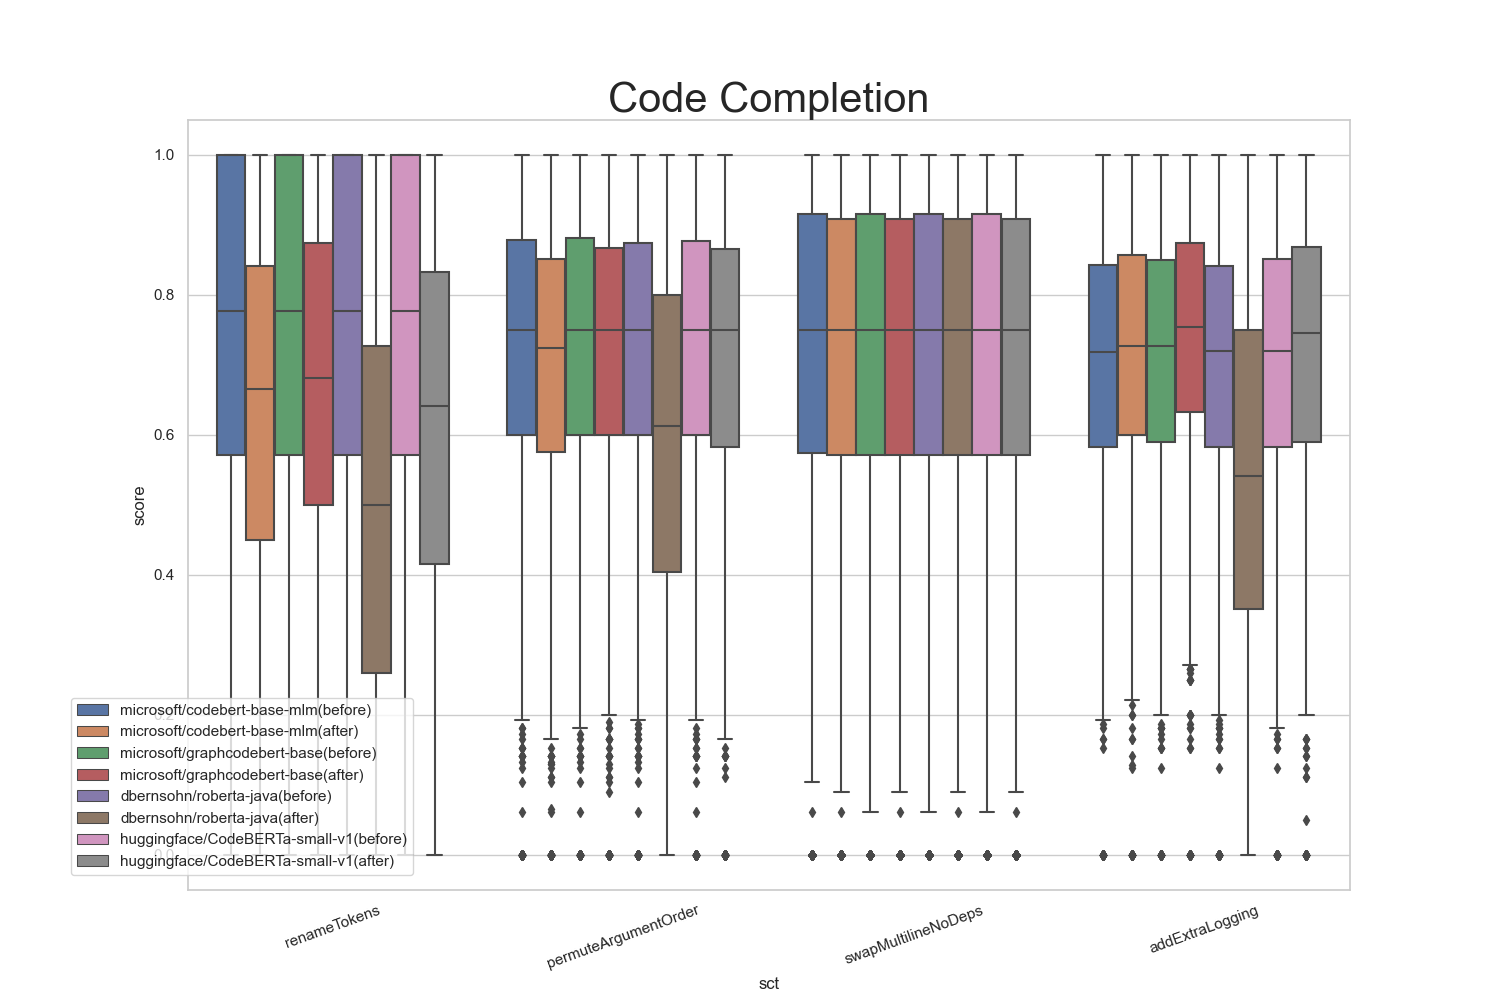
\includegraphics[width=0.38\textwidth]{figs/Code Completion}\hspace*{-0.6cm}
                  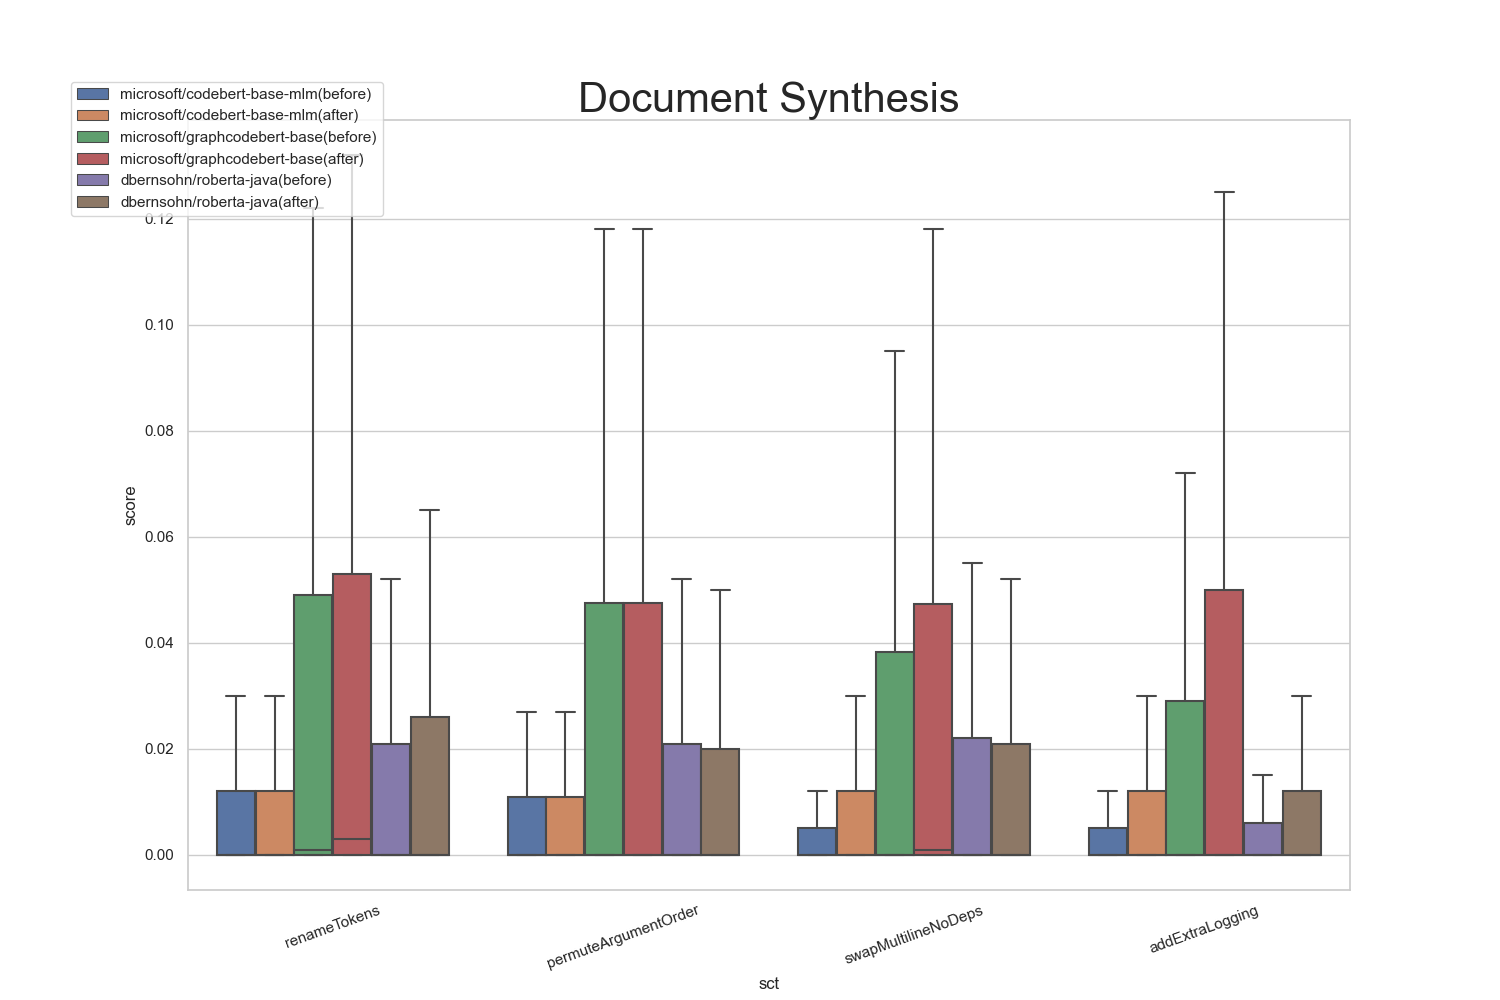
\includegraphics[width=0.38\textwidth]{figs/Document Synthesis}\hspace*{-0.6cm}
                  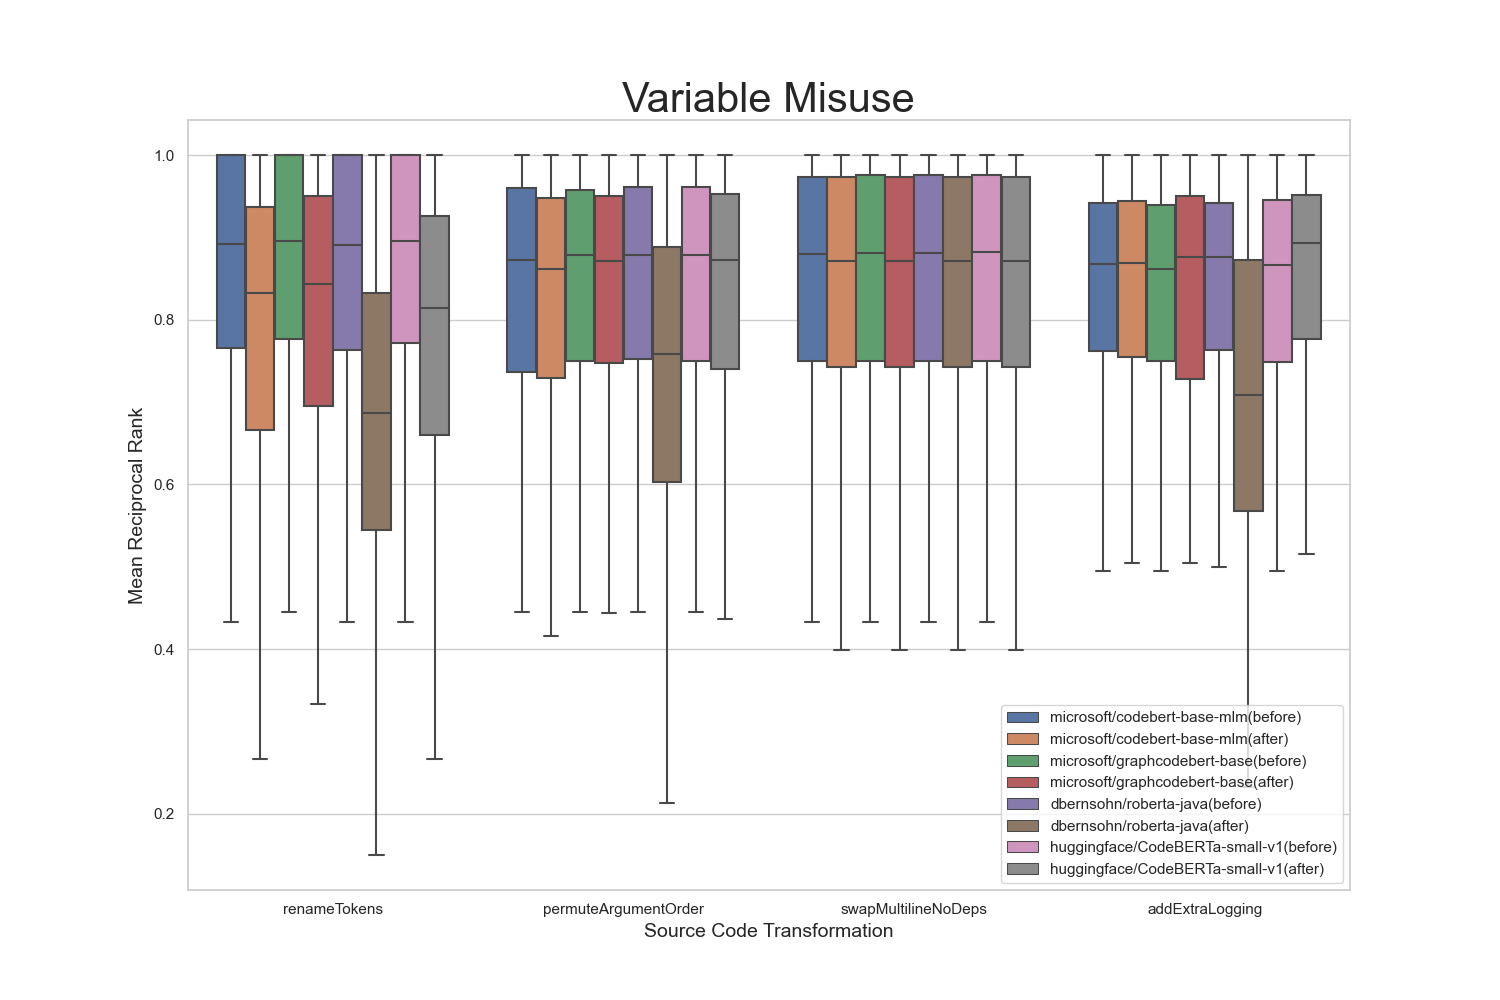
\includegraphics[width=0.38\textwidth]{figs/Variable Misuse}
                  \caption{Semantic shift across all models and transformations.}
                  \label{fig:dataflow}
  \end{figure}

  Our results support the relative model rankings as reported by prior literature: RoBERTa $\ll$ CodeBERT $<$ GraphCodeBERT. As we can see, RoBERTa is considerably more sensitive to cosmetic variance than CodeBERT and GraphCodeBERT, which are relatively close contenders. The \lstinline|swapMultilineNo| and \lstinline|permuteArgument| SCTs exhibit a more detrimental effect than the other SCTs. Unexpectedly, it appears that token renaming tends to improve completion accuracy across all models on average.

  In both cases, we observe a clear trend across method complexity: SCTs in low complexity code have a larger effect on completion quality than similar transformations in high-complexity code. We hypothesize this phenomenon can be explained by the fact that the same transformation can have a comparatively larger effect on a shorter code snippet than a longer one, which contains more contextual information and is thus more stable to minor perturbations.

  Examining the source code transformations, we notice that renaming can have a significant effect on document synthesis. As the model frequently copies tokens from the source code to the document and vis-versa, renaming tends to have a deleterious effect on document quality. Likewise, swapping multiline statements appears to have a significant negative effect on document quality.

  \section{Conclusion}\label{sec:conclusion}

  The work described herein is primarily an empirical study, but also showcases a framework and a systematic approach to evaluating neural code completion models. It offers a number of advantages from a software engineering standpoint: due to its functional implementation, it is efficient, parallelizable and highly modular, allowing others to easily reuse and extend our work with new benchmarks.

  Despite its simplicity, the regex-based SCT approach has some shortcomings. Although regular expressions are easy to implement and do support rudimentary transformations, they are a crude way to manipulate source code. In order to generate semantically valid transformations, one must really use full-fledged term rewriting system, such as higher-order abstract syntax or some kind of parser-combinator. Several options were evaluated, including OpenRewrite, TXL~\citep{cordy2004txl}, Refal~\citep{gurin1991refal} et al., but their features were ultimately found wanting (e.g., poor error recovery) and the complexity of using them (e.g., parsing, API integration) proved too burdensome.

  Our SCTs can be viewed as ``possible worlds'' in the tradition of modal logic: the original author plausibly could have chosen an alternate form of expressing the same procedure. Although we are unable to access all these worlds, we can posit the existence and likelihood of some, and given a dataset of alternate code snippets, begin to probe a candidate model's predictions.

  One intriguing avenue for future work would be to consider combinations of source code transformations. This would vastly expand the cardinality of the validation set, enabling us to access a much larger space of possible worlds, albeit potentially at the risk of lower semantic admissibility, as arbitrary combinations of SCTs can quickly produce invalid code. This presents an interesting engineering challenge and possible extension to this work.

  Although we currently only use average mutlimask accuracy and ROUGE-synonym metrics, it would be useful to incorporate various other metrics such as mean average precision (MAP), mean reciprocal rank (MRR), and normalized discounted cumulative gain (NDCG). In addition to their utility as yardstick for evaluating model robustness, these metrics can be used to retrain those same models, a direction we hope to explore in future work.

  Finally, one could imagine using the code completion model itself to generate code for testing the same model. We have implemented this functionality to a limited extent in the \textsc{AddExtraLogging} SCT, in which the model synthesizes a single token to log, and the \textsc{InsertComment} SCT, where the model inserts a short comment. While this approach could be a useful way to generate additional training data, it would would require careful monitoring and postprocessing to avoid introducing unintended feedback loops.

  Neural language models hold much promise for improved code completion, however complacency can lead to increased reviewer burden or more serious technical debt if widely adopted. While trade secrecy may prevent third-party inspection of pretrained models, users would still like some assurance of the model's robustness to naturally-occurring variance. Our work helps to address this use case, treating the model as a black box: it does not require direct access to the model parameters or training data.

  Our contributions in this work are twofold: we demonstrate that SoTA neural language models for source code, despite their effectiveness on long-range sequence prediction tasks, are unpredictable in the presence of specifically-constructed cosmetic variation. We also describe a systematic approach and open source implementation of a newly-developed software toolkit which allows users to empirically probe a candidate model's robustness to various categories of syntactic and semantic source code transformations.
  \pagebreak\bibliography{iclr2022_conference}
  \bibliographystyle{plain}
  \appendix
  \section{Detailed Results}\label{sec:detailed_results}
  We ran three tasks, code completion, documentation synthesis and variable misuse.

  \begin{center}
    \begin{table}[H]
      \resizebox{\textwidth}{!}{%
        \begin{tabular}{r|cccc}
          Pretrained Language Model  ($\mu$, $\sigma$)                       & \textsc{Rename}                  & \textsc{PermuteArgument}               & \textsc{SwapIndepLines}               & \textsc{AddExtraLogging}               \\\hline\\
          microsoft/codebert-base-mlm \stackanchor{Before}{After}   & \stackanchor{(0.7224, 0.2768)}{(0.6100, 0.3085)} & \stackanchor{(0.7194, 0.2191)}{(0.6978, 0.2227)} & \stackanchor{(0.7089, 0.2624)}{(0.7058, 0.2607)} & \stackanchor{(0.6996, 0.2077)}{(0.7122, 0.2001)}\\\\
          microsoft/graphcodebert-base \stackanchor{Before}{After}   & \stackanchor{(0.7230, 0.2767)}{(0.6410, 0.2998)} & \stackanchor{(0.7227, 0.2173)}{(0.7154, 0.2169)} & \stackanchor{(0.7088, 0.2624)}{(0.7058, 0.2607)} & \stackanchor{(0.7050, 0.2047)}{(0.7382, 0.1932)}\\\\
          dbernsohn/roberta-java \stackanchor{Before}{After}   & \stackanchor{(0.7219, 0.2773)}{(0.4951, 0.3165)} & \stackanchor{(0.7196, 0.2188)}{(0.5995, 0.2632)} & \stackanchor{(0.7087, 0.2624)}{(0.7058, 0.2607)} & \stackanchor{(0.6958, 0.2095)}{(0.5479, 0.2577)}\\\\
          huggingface/CodeBERTa-small-v1 \stackanchor{Before}{After}   & \stackanchor{(0.7226, 0.2771)}{(0.5953, 0.3134)} & \stackanchor{(0.7216, 0.2149)}{(0.7096, 0.2249)} & \stackanchor{(0.7088, 0.2624)}{(0.7058, 0.2607)} & \stackanchor{(0.7004, 0.2095)}{(0.7113, 0.2119)}\\\\
        \end{tabular}
      }
      \caption{\label{tab:code-comp}Mean and standard deviation for single-token code completion accuracy.}
    \end{table}
  \end{center}


  \begin{center}
    \begin{table}[H]
      \resizebox{\textwidth}{!}{%
        \begin{tabular}{r|cccc}
          Pretrained Language Model  ($\mu$, $\sigma$)                       & \textsc{Rename}                  & \textsc{PermuteArgument}               & \textsc{SwapIndepLines}               & \textsc{AddExtraLogging}               \\\hline\\
          microsoft/codebert-base-mlm \stackanchor{Before}{After}   & \stackanchor{(0.0385, 0.2684)}{(0.0430, 0.2996)} & \stackanchor{(0.0427, 0.3500)}{(0.0411, 0.3091)} & \stackanchor{(0.0309, 0.2477)}{(0.0419, 0.2959)} & \stackanchor{(0.0545, 0.4637)}{(0.0510, 0.3839)}\\\\

          microsoft/graphcodebert-base \stackanchor{Before}{After}   & \stackanchor{(0.0987, 0.3826)}{(0.1026, 0.3590)} & \stackanchor{(0.0983, 0.3214)}{(0.0982, 0.3212)} & \stackanchor{(0.0891, 0.4181)}{(0.0989, 0.3549)} & \stackanchor{(0.0850, 0.3000)}{(0.0974, 0.2221)}\\\\

          dbernsohn/roberta-java \stackanchor{Before}{After}   & \stackanchor{(0.0827, 0.5086)}{(0.0891, 0.5484)} & \stackanchor{(0.0727, 0.4453)}{(0.0781, 0.4792)} & \stackanchor{(0.0793, 0.4769)}{(0.0845, 0.5428)} & \stackanchor{(0.0680, 0.5349)}{(0.0733, 0.4994)}\\\\

          huggingface/CodeBERTa-small-v1 \stackanchor{Before}{After}   & \stackanchor{(0.1101, 0.3932)}{(0.1143, 0.3645)} & \stackanchor{(0.1205, 0.4148)}{(0.1170, 0.3668)} & \stackanchor{(0.0997, 0.3912)}{(0.1125, 0.3811)} & \stackanchor{(0.1252, 0.5175)}{(0.1230, 0.3891)}\\\\
        \end{tabular}
      }
      \caption{\label{tab:doc-synth}Mean and standard deviation ROUGE-score for document synthesis.}
    \end{table}
  \end{center}

  \begin{center}
    \begin{table}[H]
      \resizebox{\textwidth}{!}{%
        \begin{tabular}{r|cccc}
          Pretrained Language Model  ($\mu$, $\sigma$)                       & \textsc{Rename}                  & \textsc{PermuteArgument}               & \textsc{SwapIndepLines}               & \textsc{AddExtraLogging}               \\\hline\\
          microsoft/codebert-base-mlm \stackanchor{Before}{After}   & \stackanchor{(0.8150, 0.2502)}{(0.7508, 0.2663)} & \stackanchor{(0.7692, 0.2947)}{(0.7574, 0.2992)} & \stackanchor{(0.7935, 0.2683)}{(0.7861, 0.2720)} & \stackanchor{(0.7568, 0.3086)}{(0.7412, 0.3297)}\\\\

          microsoft/graphcodebert-base \stackanchor{Before}{After}   & \stackanchor{(0.8196, 0.2478)}{(0.7638, 0.2638)} & \stackanchor{(0.7758, 0.2873)}{(0.7673, 0.2919)} & \stackanchor{(0.7952, 0.2670)}{(0.7861, 0.2720)} & \stackanchor{(0.7529, 0.3071)}{(0.7378, 0.3376)}\\\\

          dbernsohn/roberta-java \stackanchor{Before}{After}   & \stackanchor{(0.8149, 0.2486)}{(0.6708, 0.2282)} & \stackanchor{(0.7727, 0.2947)}{(0.7148, 0.2399)} & \stackanchor{(0.7952, 0.2670)}{(0.7861, 0.2720)} & \stackanchor{(0.7620, 0.3053)}{(0.6797, 0.2580)}\\\\

          huggingface/CodeBERTa-small-v1 \stackanchor{Before}{After}   & \stackanchor{(0.8182, 0.2480)}{(0.7569, 0.2334)} & \stackanchor{(0.7736, 0.2934)}{(0.8023, 0.2318)} & \stackanchor{(0.7954, 0.2670)}{(0.7861, 0.2720)} & \stackanchor{(0.7578, 0.3053)}{(0.8137, 0.2413)}\\\\
        \end{tabular}
      }
      \caption{\label{tab:var-misuse}Mean and standard deviation MRR for variable misuse detection.}
    \end{table}
  \end{center}

  \section{Tokenization}
  Let $\Sigma$ be any alphabet (in practice, CodeBERT uses UTF-8 although it is possible to encode Chinese by switching to UTF-16).
  Let $\texttt{dict} \subset \Sigma^*\leftrightarrow\mathbb Z$ be a bijection between certain strings over $\Sigma$ and the integers.
  Let bpe: $\Sigma^*\rightarrow\mathbb{Z}^*$ be an encoder that maps strings $\Sigma^*$ to a list of integers $\mathbb{Z}^*$.
  \texttt{bpe} is defined as follows: $\texttt{bpe(s)} := \texttt{dict(s[1:p])} \oplus \texttt{bpe(s[p+1:|s|])}$ where $p = max \{ i \in \texttt{(1,|p|]} | \texttt{s[1:i]} \in \texttt{dict} \}$, $\oplus$ denotes list concatenation and $s[a:b]$ denotes the substring of s between indices a and b using 1-based indexing.
  dict has the following property: $\forall s \in \Sigma^*, bpe(s) = [i_1, i_2, \ldots, i_n]$ implies $\texttt{dict}^{-1}(i_1) \oplus \texttt{dict}^{-1}(i_2) \oplus \texttt{dict}^{-1}(\ldots) \oplus \texttt{dict}^{-1}(i_n) = s$, i.e., bpe is a lossless compression scheme.
  Furthermore, dict typically has the property that $\mathbb{E}[|bpe(s)|] \ll \mathbb{E}[|s|]$ over $s \in L \subset \Sigma^*$ where L is a language (e.g., NL or PL) in $\Sigma^*$, n.b. this is untrue if $\Sigma^*$ due to the pigeonhole principle.
%  \section{Appendix}
\end{document}
